\documentclass[12pt]{article}
\usepackage[a4paper]{geometry}
\usepackage[estonian]{babel} 
\usepackage[utf8]{inputenc}
\usepackage{nameref}
\usepackage{fancyhdr}
\PassOptionsToPackage{hyphens}{url}\usepackage{hyperref}
\usepackage{caption}
\usepackage{csquotes}
\usepackage{indentfirst}
\usepackage[biblabel]{cite}
\usepackage{boldline}
\usepackage{graphicx}
\usepackage{float}
\usepackage{listings}
\usepackage{eurosym}
%\renewcommand{\contentsname}{Sisukord}
\addto\captionsestonian{\renewcommand{\refname}{Kasutatud materjalid}}
\renewcommand{\thesection}{\arabic{section}}
% Page numbers to the right
\pagestyle{fancy}
\fancyhead{}
\fancyfoot{}
\fancyfoot[R]{\thepage}
\renewcommand{\headrulewidth}{0pt}
% Code formatting
\newcommand{\code}[1]{\texttt{#1}}

\title{Versiooniuuenduse automatiseerimine kasutades skriptimiskeelt Bash}
\author{Irina Ivanova}
\date{January 2016}

\begin{document}
  \begin{titlepage}
    \begin{center}
      TARTU ÜLIKOOL\\
      Arvutiteaduse instituut\\
      Infotehnoloogia eriala
    \end{center}
      
    \vspace{5cm}
    
    \begin{center}  
      {\Large Irina Ivanova}
    \end{center}
    \begin{center}      
      {\huge Versiooniuuenduse automatiseerimine}
    \end{center}
    \begin{center}
      {\huge kasutades skriptimiskeelt Bash}
    \end{center}
    \begin{center}
      {\large Bakalaureusetöö (6 EAP)}
    \end{center}
      
    \vspace{4cm}
    \hspace{4.5cm}
    Juhendajad: dotsent Helle Hein
    
    \hspace{7cm}
    Polina Morozova, MSc (Nortal AS)
      
    \vspace{2.5cm}
    \begin{center}
      Tartu 2016
    \end{center}
  \end{titlepage}

  \newpage
  
  \noindent\textbf{Versiooniuuenduse automatiseerimine kasutades skriptimiskeelt Bash}\\
  
  \noindent\textbf{Lühikokkuvõte:}\\
  Modulaarset süsteemi kasutavas projektis tehakse rakendusse palju uuendusi, eriti kui seda rakendust kasutavad mitu klienti. Manuaalne versioonivahetuse protsess võtab palju aega ja suurendab inimliku vea tekkimise tõenäosust. Bakalaureusetöö teoreetilise osa eesmärk on leida võimalikud lahendused uuendamisprotsessi automatiseerimiseks ja valida neist välja parim. Töö praktilise osa eesmärk on valitud lahenduse loomine ja selle rakendamine projektis.\\
  
  \noindent\textbf{Võtmesõnad:}\\
  Bash skript, versiooniuuendus, Apache Tomcat, Java, modulaarne süsteem\\
  
  \noindent\textbf{CERCS:}\\
  CERCS P170 Arvutiteadus, arvutusmeetodid, süsteemid, juhtimine (automaatjuhtimisteooria)
  \vspace{2cm}

  \noindent\textbf{Version Update Automation Using Scripting Language Bash}\\

  \noindent\textbf{Abstract:}\\
  There are a lot of application updates in a project, where modular system is in use, especially if the application is used by many clients. Manual version update process takes a lot of time and increases the possibility of human errors. The aim of the theoretical part of this Bachelor's Thesis is to find possible solutions for the application update process automation and to choose the best one. The aim of the practical part is to create the solution and apply it to the project.\\

  \noindent\textbf{Keywords:}\\
  Bash script, version update, Apache Tomcat, Java, modular system\\
  
  \noindent\textbf{CERCS:}\\
  CERCS P170 Computer science, numerical analysis, systems, control
  
  \newpage
 
  \tableofcontents
  \fancypagestyle{plain}{%
    \renewcommand{\headrulewidth}{0pt}%
    \fancyhf{}%
    \fancyfoot[R]{\thepage}%
  }
 
  \newpage
  
  % Sissejuhatus
  \section*{Sissejuhatus}
  \label{sissejuhatus}
  \addcontentsline{toc}{section}{\nameref{sissejuhatus}}
  
  Tarkvara versiooniuuendamine on protsess, mille korral veebiserverisse paigaldatakse mooduli uuem versioon, et rakendada selles olemasolevaid koodiparandusi või täiendusi. Tavaliselt manuaalne uuendus koosneb neljast põhisammust: uue versiooni allalaadimine, selle paigaldamine, vana versiooni eemaldamine ja uue versiooni staatuse kontrollimine. Mida rohkem on mooduleid ja veebiservereid, seda ajamahukamaks muutub versiooniuuendamise protsess, kuna neid samme on vaja korrata mitu korda.
  
  Käesolevas lõputöös keskendutakse rakendusliku probleemi lahendamisele toimivas tarkvaraprojektis. Projekti olemuse tõttu võtab rakenduse versiooniuuendus kaua aega ja eeldab palju manuaalset sekkumist. See kulutab ressursse ja suurendab inimliku vea tekkimise tõenäosust. Bakalaureusetöö teoreetilise osa eesmärk on leida võimalikud lahendused uuendamisprotsessi automatiseerimiseks ja valida neist välja parim. Praktilise osa eesmärk on valitud lahenduse loomine ja selle rakendamine projektis.
  
  Töö koosneb viiest osast. Esimeses osas püstitatakse probleem: kirjeldatakse projekti arhitektuuri, manuaalset uuendamisprotsessi, senise protsessiga kaasnevaid probleeme ja nõudeid uuele lahendusele. Peamine raskus seisneb selles, et rakendus koosneb paarikümnest moodulist (täpne arv sõltub kliendi nõuetest), mis tuleb paigaldada 30 rakendusesse. Selleks, et paigaldada rakenduse uus versioon kõigisse veebiserveritesse, on vaja teha umbes 600 uuendust (arvestamata testrakenduste vaheuuendusi). Lisaks on projektis kasutusel kaks erinevat veebiserverit: Oracle WebLogic 12\footnote{\url{https://www.oracle.com/middleware/weblogic} (12.05.2016)} ja Apache Tomcat 8\footnote{\url{http://tomcat.apache.org} (12.05.2016)}. Uuendamisprotsessi automatiseerimine peab arvestama kõigi nende nõuetega.
  
  Töö teises osas uuritakse võimalikke lahendusi: kas kasutada turul olemasolevat toodet (töös uuritakse nelja toodet: Atlassian Bamboo, Chef, Jenkins ja Ansible Tower) või kirjutada ise tarkvara. Tuuakse välja iga lahenduse eeliseid ja puuduseid ning selgitatakse, miks langetati otsus Bash skripti kirjutamise kasuks. Valmistoodete peamised puudused on nende maksumus, võimetus hallata protsesse ja parandada vigu, vajadus kulutada palju aega toote tundmaõppimiseks ja rakendamiseks.
  
  Kolmandas osas kirjeldatakse valitud lahendust: milline on skripti tööpõhimõte ja arhitektuur ning kuidas skripti saab paigaldada ja kasutada. Skripti põhifunk\-tsioonid on moodulifaili allalaadimine, vana versiooni mahavõtmine, uue versiooni paigaldamine ja vajalike inimeste teavitamine toimunud versiooniuuendusest. Lisaks on oluliseks funktsiooniks erinevad kontrollid, mis vähendavad vale versiooni paigaldamise tõenäosust, samuti logimisfunktsioon, mis võimaldab hankida andmeid iga uuenduse kohta.
  
  Neljandas osas uuritakse, kuidas valitud lahendus mõjutas projekti: võrreldakse versiooniuuendusele kulunud aega manuaalse ja automatiseeritud protsessi puhul ning vahendatakse kolleegidelt uue uuendamisprotsessi kasutamise kohta saadud tagasisidet.
  
  Viimases osas tuuakse välja lahenduse kaugemaid perspektiive: kuidas saab loodud skripti edasi arendada ja teistes projektides rakendada.
  
  Tööl on kaheksa lisa: terminid, ühe mooduli uuendamisprotsessi mudel, mitme mooduli uuendamisprotsessi mudel, skripti projektisisene juhend, skripti avalik juhend, kolleegide tagasiside skripti kohta, Bash skripti lähtekood ja litsents.
  
  Käesoleva bakalaureusetöö tulemuseks on töötav, avatud lähtekoodiga skript Bash keeles ja selle dokumentatsioon.
  
  \newpage
  
  % Probleemi püstitus
  \section{Probleemi püstitus}
  
  Versioonide uuendamine on tarkvara arendamisel sage ja vajalik protsess. Käes\-olevas töös kirjeldatud projektis etendab see protsess väga olulist rolli.
  
  Projekti rakendus on kirjutatud Javas ja kasutusel on war\--failid. Lisaks on projektis kasutatud modulaarset süsteemi, mis tähendab, et kogu rakenduse kood on jagatud mooduliteks ja iga mooduli kohta on olemas eraldi war\--fail. Kokku on umbes 20 moodulit (täpne arv sõltub kliendist, sest eri klientidel on erinev moodulite komplekt).
  
  Rakendust kasutavad 10 klienti, kellest kolmel on olemas kolm rakendust: toode, demorakendus (kus kliendid tutvuvad enne tooteuuendust uute funktsioonide ja parandustega) ja testrakendus (kus projekti meeskond testib toote funktsioone enne selle tarnimist kliendile). Seitsmel kliendil on olemas kaks rakendust: toode ja testrakendus. See tähendab, et kokku on $3*3+7*2=23$ kliendirakendust. Lisaks on projektis veel umbes seitse testrakendust, mida kasutatakse eri faasides eri funktsioonide testimiseks. Seega tuleb kokku $23+7=30$ rakendust (arvestamata kohalikke ja virtuaalmasinaid, mida iga meeskonnaliige võib vajadusel luua), mida on samuti vaja regulaarselt uuendada. See tähendab, et rakenduse uue versiooni paigaldamiseks igasse rakendusesse on vaja teha $30*20=600$ uuendust.
  
  Toodud arvud näitavad, et versiooni manuaalne uuendamine nõuab palju aega ja tähelepanu, mistõttu otsustati uuendamisprotsessi automatiseerida.
    
  Tabelis 1 on esitatud ühe mooduli manuaalse uuendamisprotsessi sammud.
  
  \begin{table}[H]
    \caption*{\textit{Tabel 1. Manuaalse uuendamisprotsessi sammud.}}
  
    \begin{tabular}{ |c|p{11cm}| }
      \hline
      \textbf{Samm} & \textbf{Tegevus}\\
      \hline
      1 & Uue versiooninumbriga war\--faili allalaadimine serverisse.\\
      \hline
      2 & Kui veebiserveriks on Oracle WebLogic, siis war\--faili prekompileerimine (Apache Tomcat veebiserveril seda sammu ei ole).\\
      \hline
      3 & Faili ümbernimetamine.\\
      \hline
      4 & Faili paigaldus.\\
      \hline
      5 & Vana faili eemaldamine.\\
      \hline
      6 & Uue versiooni staatuse kontrollimine.\\
      \hline
      7 & JIRA\footnotemark{} töö uuendamine. JIRA saadab automaatselt kollegidele teate versiooniuuenduse kohta.\\
      \hline
      8 & Allalaaditud faili kustutamine.\\
      \hline
    \end{tabular}
  \end{table}
  
  \footnotetext{\url{https://www.atlassian.com/software/jira} (12.05.2016)}
  
  Sammus 7 mainitud JIRA põhifunktsiooniks on ülesannete haldamine. Projektis seda kasutatakse versiooniuuenduste jälgimiseks: iga mooduli ja rakenduse kohta on olemas eraldi JIRA töö (\textit{issue}), kus uuendatakse selle pealkirja (\textit{summary}) versioonivahetuse järel. Need kasutajad, kes jälgivad (\textit{watching}) selliseid töid saavad teavitusi töö pealkirja muutmise kohta. See võimaldab mitte ainult teavitada inimesi toimunud uuenduste kohta, vaid ka tekitada töölaud (\textit{dashboard}), kus on nähtavad kõik versioonid, mis on paigaldatud konkreetsetes rakendustes.
  
  Mitme mooduli uuendamisel tuleb läbida kõik sammud Tabelis 1 iga mooduli korral eraldi. Neile tegevustele kuluv aeg sõltub moodulist (kuna mõnes moodulis võib olla teistest kordades rohkem koodi, siis selle allalaadimine ja paigaldamine võtab rohkem aega), aga keskmiselt on see 1.5 minutit. Kõikide moodulite uuendamine võib võtta aega ühe tunni, sest lisandub veel aeg õige versiooninumbri leidmiseks, war\--faili aadressi kopeerimiseks, JIRA õige töö leidmiseks ja avamiseks jne. See tähendab, et inimlike vigade tekkimise tõenäosus on suur (nt mooduli vale versiooni allalaadimine).
  
  Tabelis 2 on toodud nõuded versiooniuuenduse automatiseerimiseks. Nende nõuete kehtestamisel on peetud silmas, et tulemuseks oleks lahendus, millesse on mõtet aega investeerida, sest uue protsessi loomine on ajamahukas tegevus ja sellest saadav tulu peab olema suurem sellele kulutatud ajast.
  
  \begin{table}[H]
    \caption*{\textit{Tabel 2. Nõuded versiooniuuenduse lihtsustamise lahendusele.}}
    
    \begin{tabular}{|c|p{3.5cm}|p{9cm}|}
      \hline
      \textbf{Nr} & \textbf{Nõue} & \textbf{Kirjeldus}\\
      \hline
      1 & Kiirus. & Uuendamisprotsess peab võtma varasemast vähem aega.\\
      \hline
      2 & Mugavus. & Uuendamisprotsess peab eeldama võimalikult vähe käsitsi tegevusi.\\
      \hline
      3 & Ühe ja mitme mooduli uuendamine. & Lahendus peab võimaldama nii ühe kui ka mitme mooduli samaaegset uuendamist.\\
      \hline
      4 & Töötamine erinevatel veebiserveritel. & Projekt kasutab kahte erinevat veebiserverit: Apache Tomcat 8 ja Oracle WebLogic 12.\\
      \hline
      5 & Teavitussüsteem. & Meeskonnaliikmed soovivad saada tehtud uuenduste kohta teavitusi.\\
      \hline
      6 & Logimissüsteem. & Peab olema võimalus vaadata, kes ja millal uuendas mingit moodulit mingis rakenduses.\\
      \hline
      7 & Mittetehniline kasutus. & Lahenduse kasutamine ei tohi nõuda erilisi tehnilisi teadmisi.\\
      \hline
      8 & Lukustamissüsteem. & Uuendustega võib tegeleda samaaegselt mitu inimest, mis tähendab, et lahendusel peab olema lukustamissüsteem, vältimaks paralleelseid uuendusi samas serveris.\\
      \hline
      9 & Töötamine mitme serveriga. & Rakendused kasutavad kahte serverit, seega peab lahendus oskama uuendada versiooni automaatselt kahel serveril.\\
      \hline
      10 & Hallatav lahendus. & Lahendus peab olema täielikult projekti kontrolli all, et seda oleks võimalik igal ajal hallata, seadistada ja parandada.\\
      \hline
      11 & Kiire arendusprotsess. & Lahenduse loomine ei tohi võtta palju aega, sest projektil puuduvad selleks inimressursid.\\
      \hline
      12 & Töötamine moodulite erisufiksitega. & Projektis on olemas Eesti ja Leedu rakendused, kuhu paigaldatakse samad moodulid, aga erinevate sufiksitega. Näiteks, kui Eesti rakenduses paigaldatakse moodulit \code{person}, siis Leedu rakenduses \code{person-lt}, kuna seal on olemas eriloogika Leedu isikute jaoks.\\
      \hline
      13 & Madal hind. & Lahendus ei tohi võtta palju raha.\\
      \hline
    \end{tabular}
  \end{table}
  
  \newpage
  
  % Võimalikud lahendused
  \section{Võimalikud lahendused}
  
  Uuendamisprotsesside automatiseerimiseks ja haldamiseks on olemas palju valmistooteid. Töös vaadeldatakse neli: Atlassian Bamboo \cite{bamboo}, Chef \cite{chef}, Jenkins \cite{jenkins} ja Ansible Tower \cite{ansible}.
  
  Kõigi valmistoodete rakendamisel on alati nii eeliseid kui ka puudusi. Valmistoodete eelisteks on:
  \begin{itemize}
    \item ei ole vaja kulutada aega juba olemasoleva süsteemi kirjutamisele;
    \item turul olevate populaarsete rakenduste puhul on suur tõenäosus, et need on kvaliteetsed ja vastavad kasutajate ootustele;
    \item vajadusel saab rakendada konkreetse tarkvara kasutajate kogukonna oskusteavet, abi ja kogemusi.
  \end{itemize}
  
  Olemasolevate süsteemide rakendamisel on ka terve rida puudusi:
  \begin{itemize}
    \item suurem osa valmistoodetest on tasulised (Jenkins on erandiks) ning nende hind tavaliselt sõltub serverite, rakenduste ja moodulite arvust, mis vaadeldavas projektis on suur;
    \item valmistoote tundmaõppimine, selle paigaldamine ja seadistamine võtab palju aega, eriti kui see pakub laia funktsioonide valikut;
    \item projekti töö sõltub tootjast \--- vigade ilmnemisel ei saa olla kindel kas ja millal need parandatakse; probleemide tekkimisel ei saa olla kindel, et tootja suudab pakkuda kasutajatuge;
    \item projekt peab usaldama tootjat \--- kui toode kood ei ole avalik, siis ei saa kontrollida selle turvalisust ja jõudlust.
  \end{itemize}
    
  Alternatiiv valmistoote kasutamisele on kirjutada oma lahendus. Kuna selline lahendus peab suhtlema teiste veebiteenustega ja töötama kõikides operatsioonisüsteemides sama moodi, siis valiti antud juhul lahenduse aluseks skriptimiskeel Bash \cite{bash,bash-book}, mis on kõige mugavam veebiteenustega töötamiseks.
  
  Tabelis 3 on toodud valmistoodete vastavus Tabelis 1 esitatud nõuetele. Kõige olulisem on 11. nõue, mille kohaselt ``lahenduse loomine ei tohi võtta palju aega, sest projektil puuduvad selleks inimressursid''.
  
  \begin{table}[H]
    \caption*{\textit{Tabel 3. Võimalike lahenduste vastavus nõuetele.}}
    
    \begin{tabular}{ |l|c|c|c|c|c|c|c|c|c|c V{4} c V{4} c|c| }
      \clineB{12-12}{4}
      \hline
      \textbf{Lahendus / Nõude Nr} & \textbf{1} & \textbf{2} & \textbf{3} & \textbf{4} & \textbf{5} & \textbf{6} & \textbf{7} & \textbf{8} & \textbf{9} & \textbf{10} & \textbf{11} & \textbf{12} & \textbf{13}\\
      \hline
      Atlassian Bamboo & x & x & x & x & x & x & x & x & x & & & x & x\\
      \hline
      Chef & x & x & x & x & x & x & x & x & x & & & x &\\
      \hline
      Jenkins & x & x & x & x & x & x & x & x & x & x & & x & x\\
      \hline
      Ansible Tower & x & x & x & x & x & x & x & x & x & & & x & \\
      \hline
      Bash skript & x & x & x & x & x & x & x & x & x & x & x & x & x\\
      \clineB{12-12}{4}
      \hline
    \end{tabular}
  \end{table}

  Atlassian Bamboo nõuab erilist tähelepanu, kuna projektis kasutatakse teisi Atlassiani tooteid, nagu JIRA, Confluence\footnote{\url{https://www.atlassian.com/software/confluence} (12.05.2016)} ja Fisheye\footnote{\url{https://www.atlassian.com/software/fisheye} (12.05.2016)}. See tähendab esiteks, et Bamboo on antud projekti jaoks tasuta (tavaliselt on see tasuline), teiseks, Bamboo integreerub väga hästi projektiga, võimaldades luua seoseid rakenduse koodi, muudatuste kirjelduse ja uuenduste vahel. Lisaks, kasutavad antud toodet ka ettevõtte teised projektid, mis annab võimaluse kaasata inimesi, kellel on olemas teadmised ja kogemused Bamboo seadistamisest.
  
  Teadmised aitavad seda rakendada võimalikult kiiresti, kuid kogemus näitas, et Bamboo lõplik rakendamine võttis teistes projektides siiski palju aega: näiteks, kulus ühes projektis ühe mooduli seadistamisele 1.5 kuud, mis 20 mooduli korral tähendaks $\sim20*1.5 \approx 30$ kuud. Lisaks võib võtta üks uuendus palju aega, sest Bamboo tööpõhimõte eeldab kolmanda serveri kasutamist uuenduse tööplaani teostamiseks ja selliste serverite arv on piiratud. See tähendab, et kui korraga soovitakse uuendada mitut rakendust, siis võib tekkida ootejärjekord.
  
  Chef ja Ansible Tower ei täida nõuded 10, 11 ja 13 \--- projekt ei saa neid kontrolleerida, nad nõuavad palju aega tundmaõppimiseks ja seadistamiseks (ettevõtes puudub vastav kogemus) ja nad nõuavad palju raha. Näiteks, Ansible Tower Premium\footnote{\url{https://www.ansible.com/pricing} (12.05.2016)} pakub ööpäevaringset kliendituge, 100 sõlme (\textit{node}) ja maksab \euro 12,286 (\$14,000)\footnote{Mõlemad Ansible Tower ja Chef hinnad on arvutatud kasutades Eesti panga eurokurssi kalkulaatorit veebilehel \url{http://www.eestipank.ee/valuutakursid} (10.05.2016).} aastas. Chef Premium\footnote{\url{https://www.chef.io/pricing} (12.05.2016)} pakub ööpäevaringset kliendituge ja \euro 111.45 (\$127) aastas ühe sõlme eest, mis 100 sõlme korral on \euro 11,145.24 (\$12,700).
  
  Jenkins ei vasta kõige olulisemale nõudele 11 \--- võtab aega tootega tutvumiseks ja selle rakendamiseks. Kuna uuendus ei tegele ainult war\--faili paigaldamisega, vaid ka selle kokkupanemisega (\textit{build}), see tähendab, et projektis on vaja lisaks muuta versioonide kokkupanemise protsessi. Sellega kaasneb suurem inimressurss, mis tähendab rohkem kulusid.
  
  \newpage
  
  Kõige sobilikum oleks uue Bash skripti kirjutamine, kuna see on ainus lahendus, mis vastab kõikidele nõuetele ja, mis kõige olulisem, sealhulgas ka 11. nõudele. Võrreldes Bamboo lahendusega on sellel valikul ka üks puudus: seda ei saa integreerida teiste Atlassiani toodetega. Samas on sellel lahendusel ka oma lisaeelised.
  \begin{itemize}
    \item Skripti on võimalik arendada osade kaupa: alguses luua lihtsamad funktsioonid, mida hiljem saab järk\--järgult täiendada uute ja keerulisemate funktsioonidega. See võimaldab kasutada ressursse väikeste osadena ja samal ajal töötada parema süsteemiga.
    \item Lahendus on väga paindlik: saab arendada konkreetsele projektile vajalikke funktsioone ning lisada seadistamise võimalus, et sama lahendust saaks kasutada erinevates serverites ja rakendustes.
    \item Lahendus ei nõua projekti arhitektuuri ja protsesside muutmist: arendajate jaoks uue versiooni loomise protsess jääb samaks.
  \end{itemize}
  
  Arvestades kõikide lahenduste eeliseid ja puudusi, otsustati Bash skripti kirjutamise kasuks.
  
  \newpage
  
  % Versiooniuuenduse automatiseerimine kasutades skriptimiskeelt Bash
  \section{Versiooniuuenduse automatiseerimine kasutades skriptimiskeelt Bash}
  
  \subsection{Lahenduse arhitektuur ja tööpõhimõte}
  
  Skript automatiseerib kõik tegevused Tabelis 1. See käivitatakse serveris, kus on vaja uuendada kas ühte või mitut moodulit ning parameetritena antakse ette mooduli nimetus, versioon ja JIRA kasutajatunnus (mitme mooduli uuendamisel mooduli nimetus ja versioon puuduvad).
  
  Joonisel 1 on näidatud protsessid, mis toimuvad ühe mooduli uuendamisel Tomcat 8 veebiserveris (faili \code{update-version-tomcat.sh} käivitamisel). Joonis on originaalkujul Lisas II.
   
   \begin{figure}[H]
     \begin{center}
       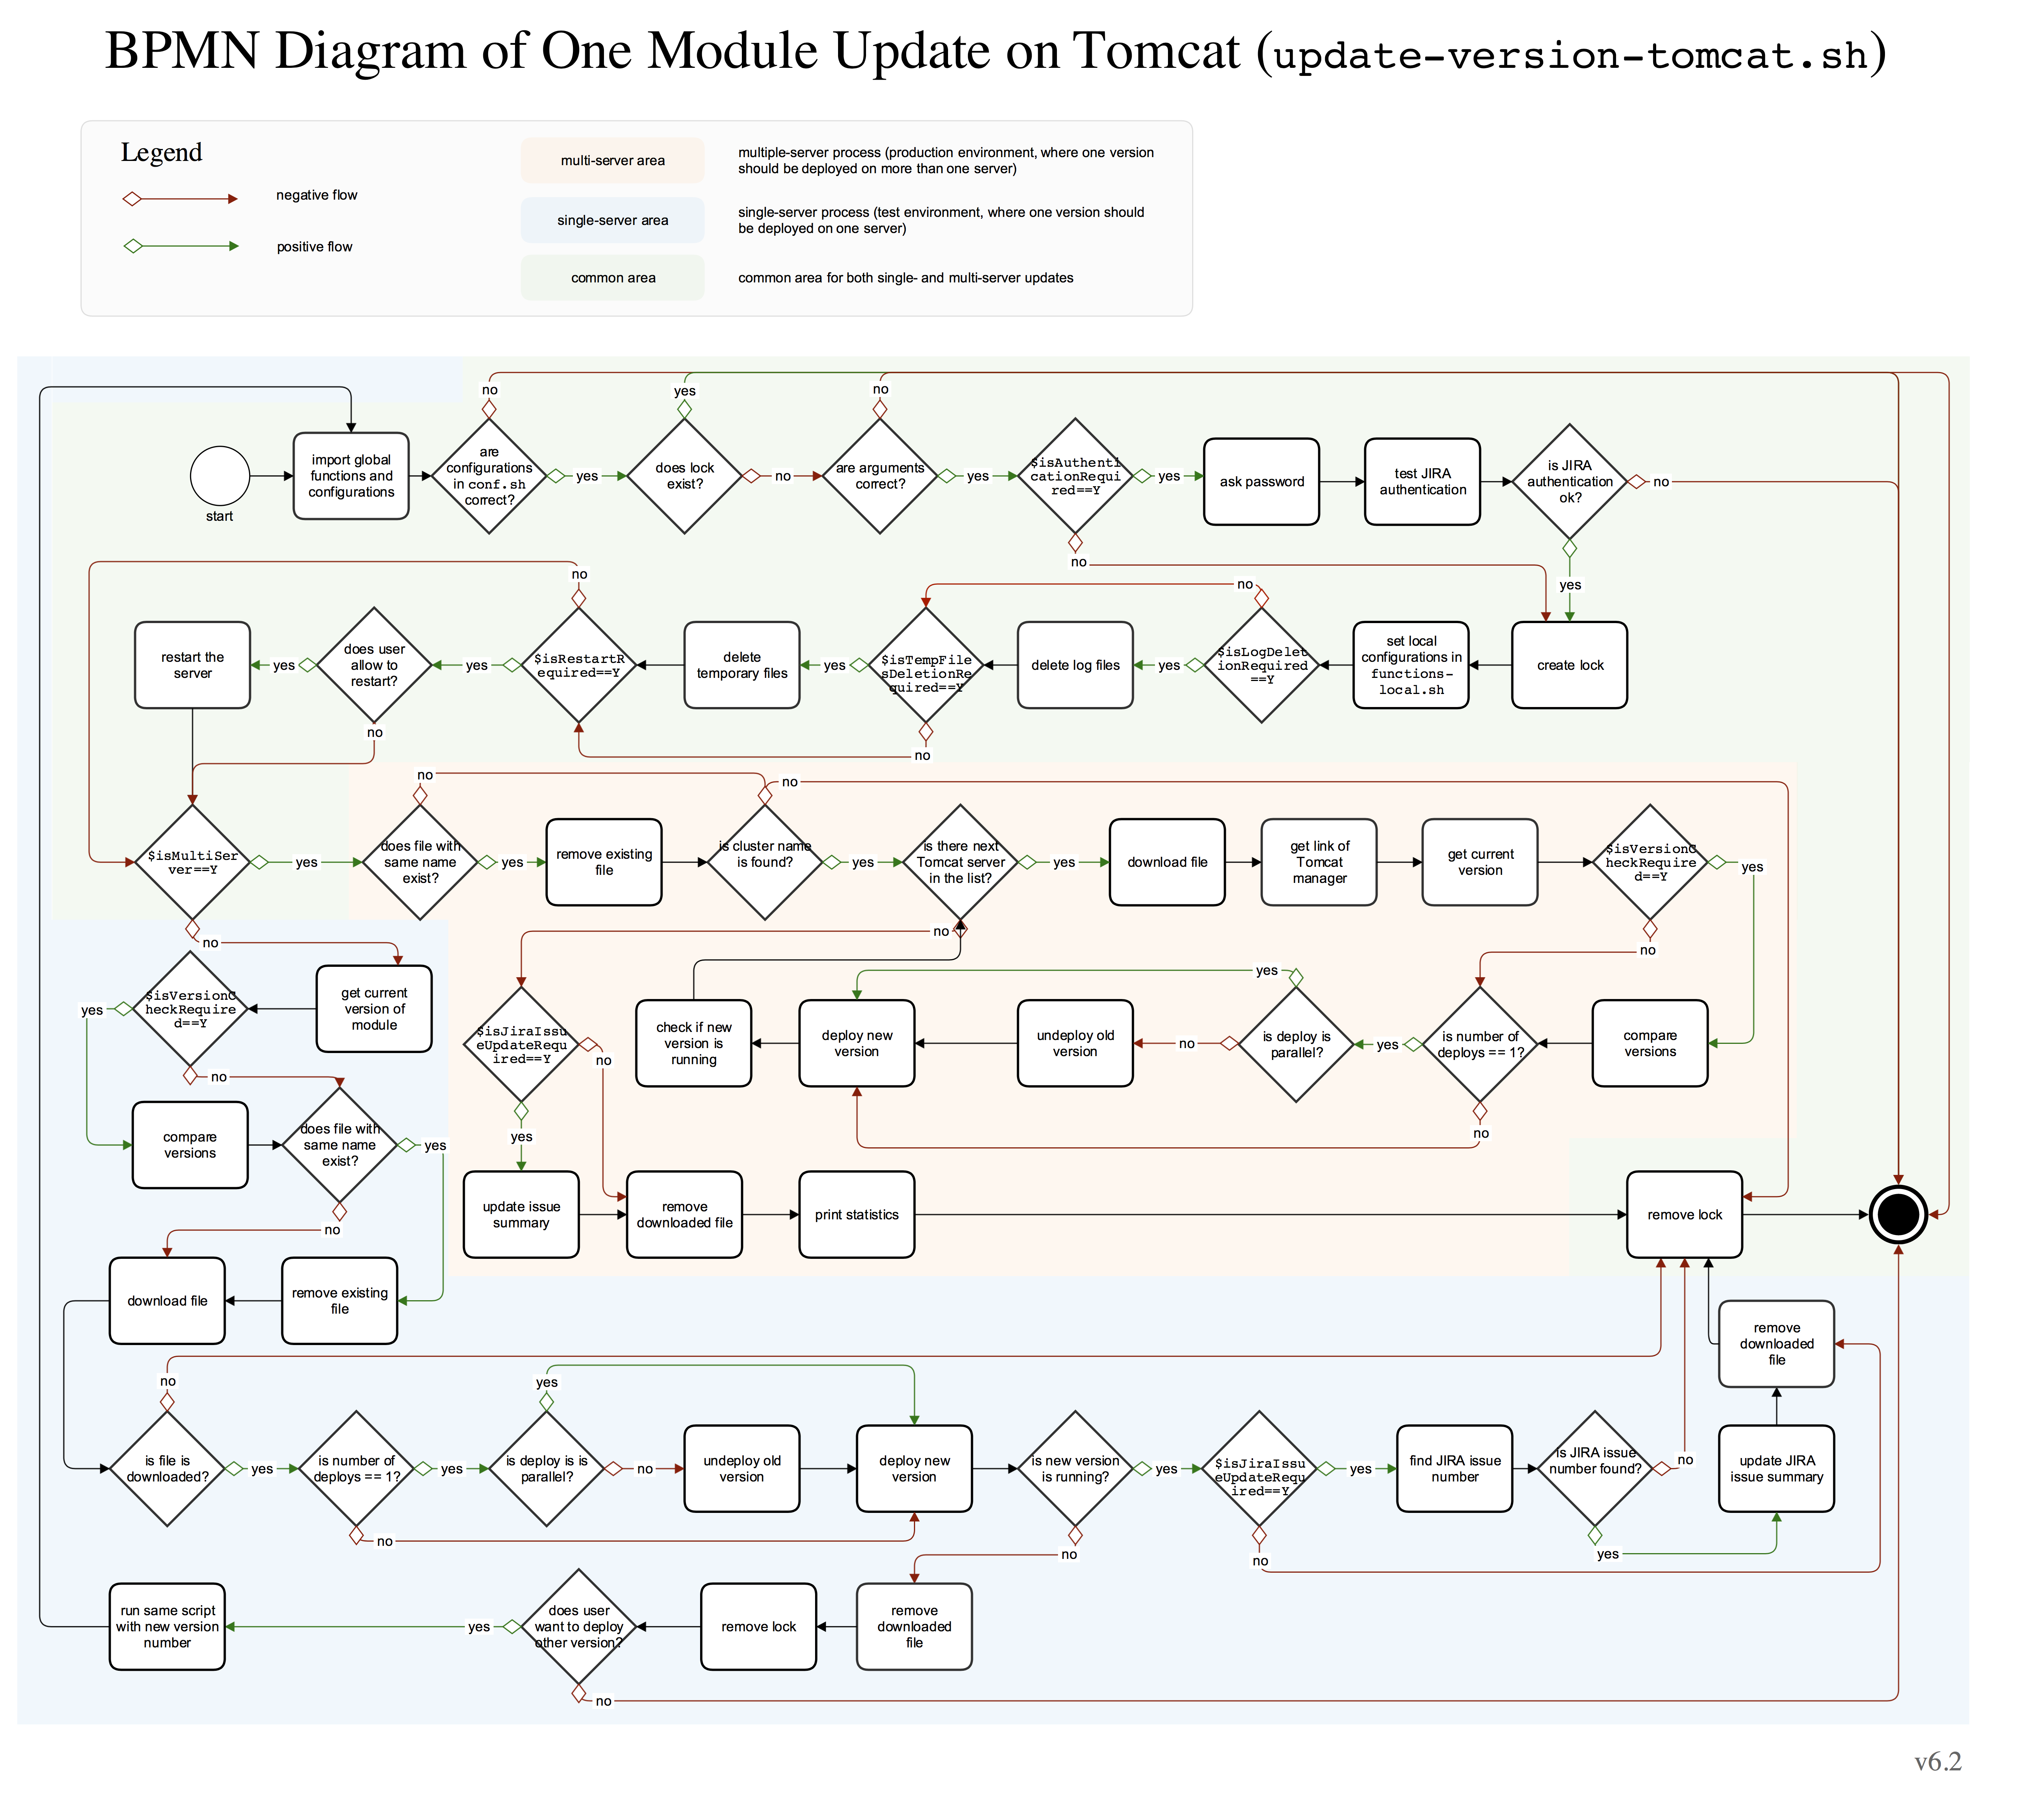
\includegraphics[width=.8\textwidth]{diagrams/BPMN-diagram-one-module-tomcat.png}
       \caption*{\textit{Joonis 1. Skripti protsessimudel ühe mooduli uuendamisel Tomcat 8 veebiserveril.}}
     \end{center}
   \end{figure}
   
   \newpage
   
   Joonisel 1 on toodud äriprotsesside mudel (\textit{Business Process Modelling Notation\footnote{\url{http://www.bpmn.org} (12.05.2016)}}), mis kirjeldab skripti teostatavaid samme ja kontrolle. Positiivsel töövool on rohelised nooled ja negatiivsel punased. Ühe mooduli uuendamisprotsess sõltub sellest, mitmes serveris uuendust tehakse: testrakendustel on üks server ja toodangurakendustel kaks serverit (skript töötab ka suurema serverite arvuga). Selle põhjal on töövoog jagatud kolmeks osaks: rohelise taustaga alal asuvad protsessid, mis on samad nii ühe kui ka mitme serveri puhul; kollasel taustal on mitme serveri protsessid ja sinisel ühe serveri protsessid. Voogude põhierinevus on kohtades, kus lõpetatakse skripti töö: nt kui mitme serveri korral ei õnnestunud mooduli paigaldamine ühes serveris, siis tuleb jätkata teise serveriga. Lisaks näidatakse mitme serveri korral töö lõpus statistikat (Joonis 2), millest selgub uuendamise seis igas serveris.
   
   \begin{figure}[H]
     \begin{center}
       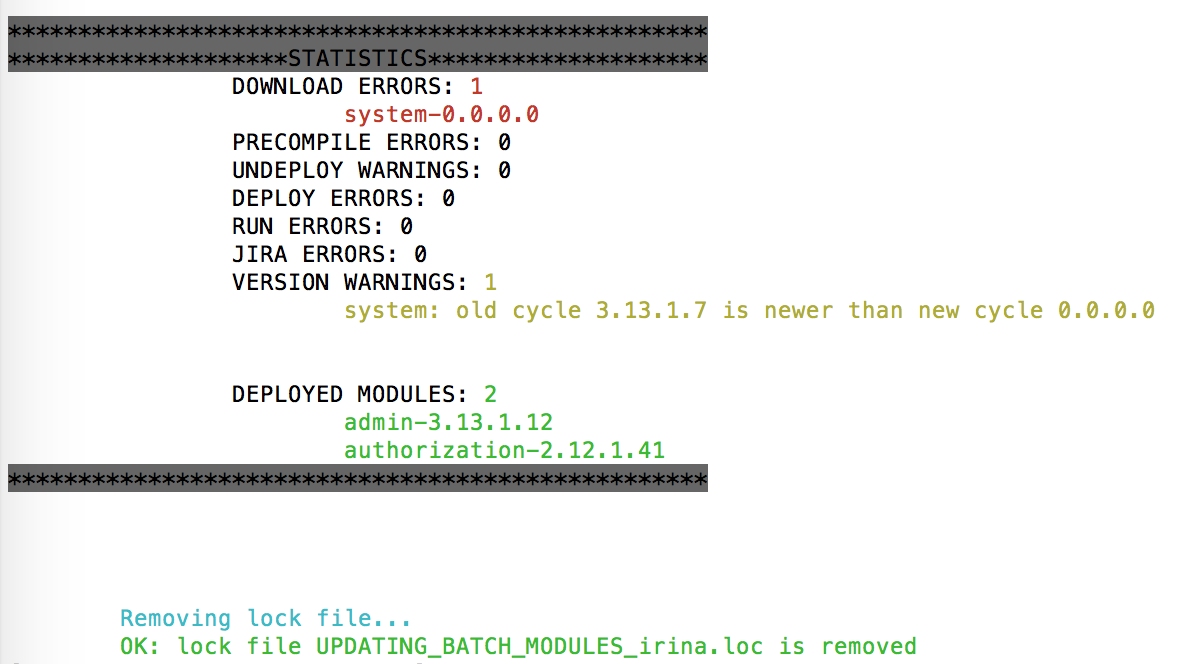
\includegraphics[width=\textwidth]{screenshots/statistics.png}
       \caption*{\textit{Joonis 2. Kolme mooduli uuendamise statistika.}}
     \end{center}
   \end{figure}
   
   Joonisel 2 on esitatud statistika, mida kuvatakse mitme mooduli uuendamisel või ühe mooduli uuendamisel mitmes serveris. See annab võimaluse aru saada uuenduse staatusest lugemata tervet teate. Antud juhul on toodud kolme mooduli \--- \code{system}, \code{admin} ja \code{authorization} \--- uuendamise statistika, mille kohaselt on  kaks moodulit edukalt uuendatud ja \code{system} mooduliga tekkis kaks probleemi: uue versiooni number \code{0.0.0.0} on väiksem vana versiooni numbrist \code{3.13.1.7} ja skriptil ei õnnestunud alla laadida uue versiooni faili nimega \code{system-0.0.0.0}. 
   
   Joonisel 3 on näidatud protsesse, mis toimuvad mitme mooduli uuendamisel Tomcat 8 veebiserveris (faili \code{batch-update-versions-tomcat.sh} käivitamisel). Sinise taustaga alal on protsessid, mis korduvad iga mooduli juures. Joonis on originaalsuuruses Lisas III.
   
   \begin{figure}[H]
     \begin{center}
       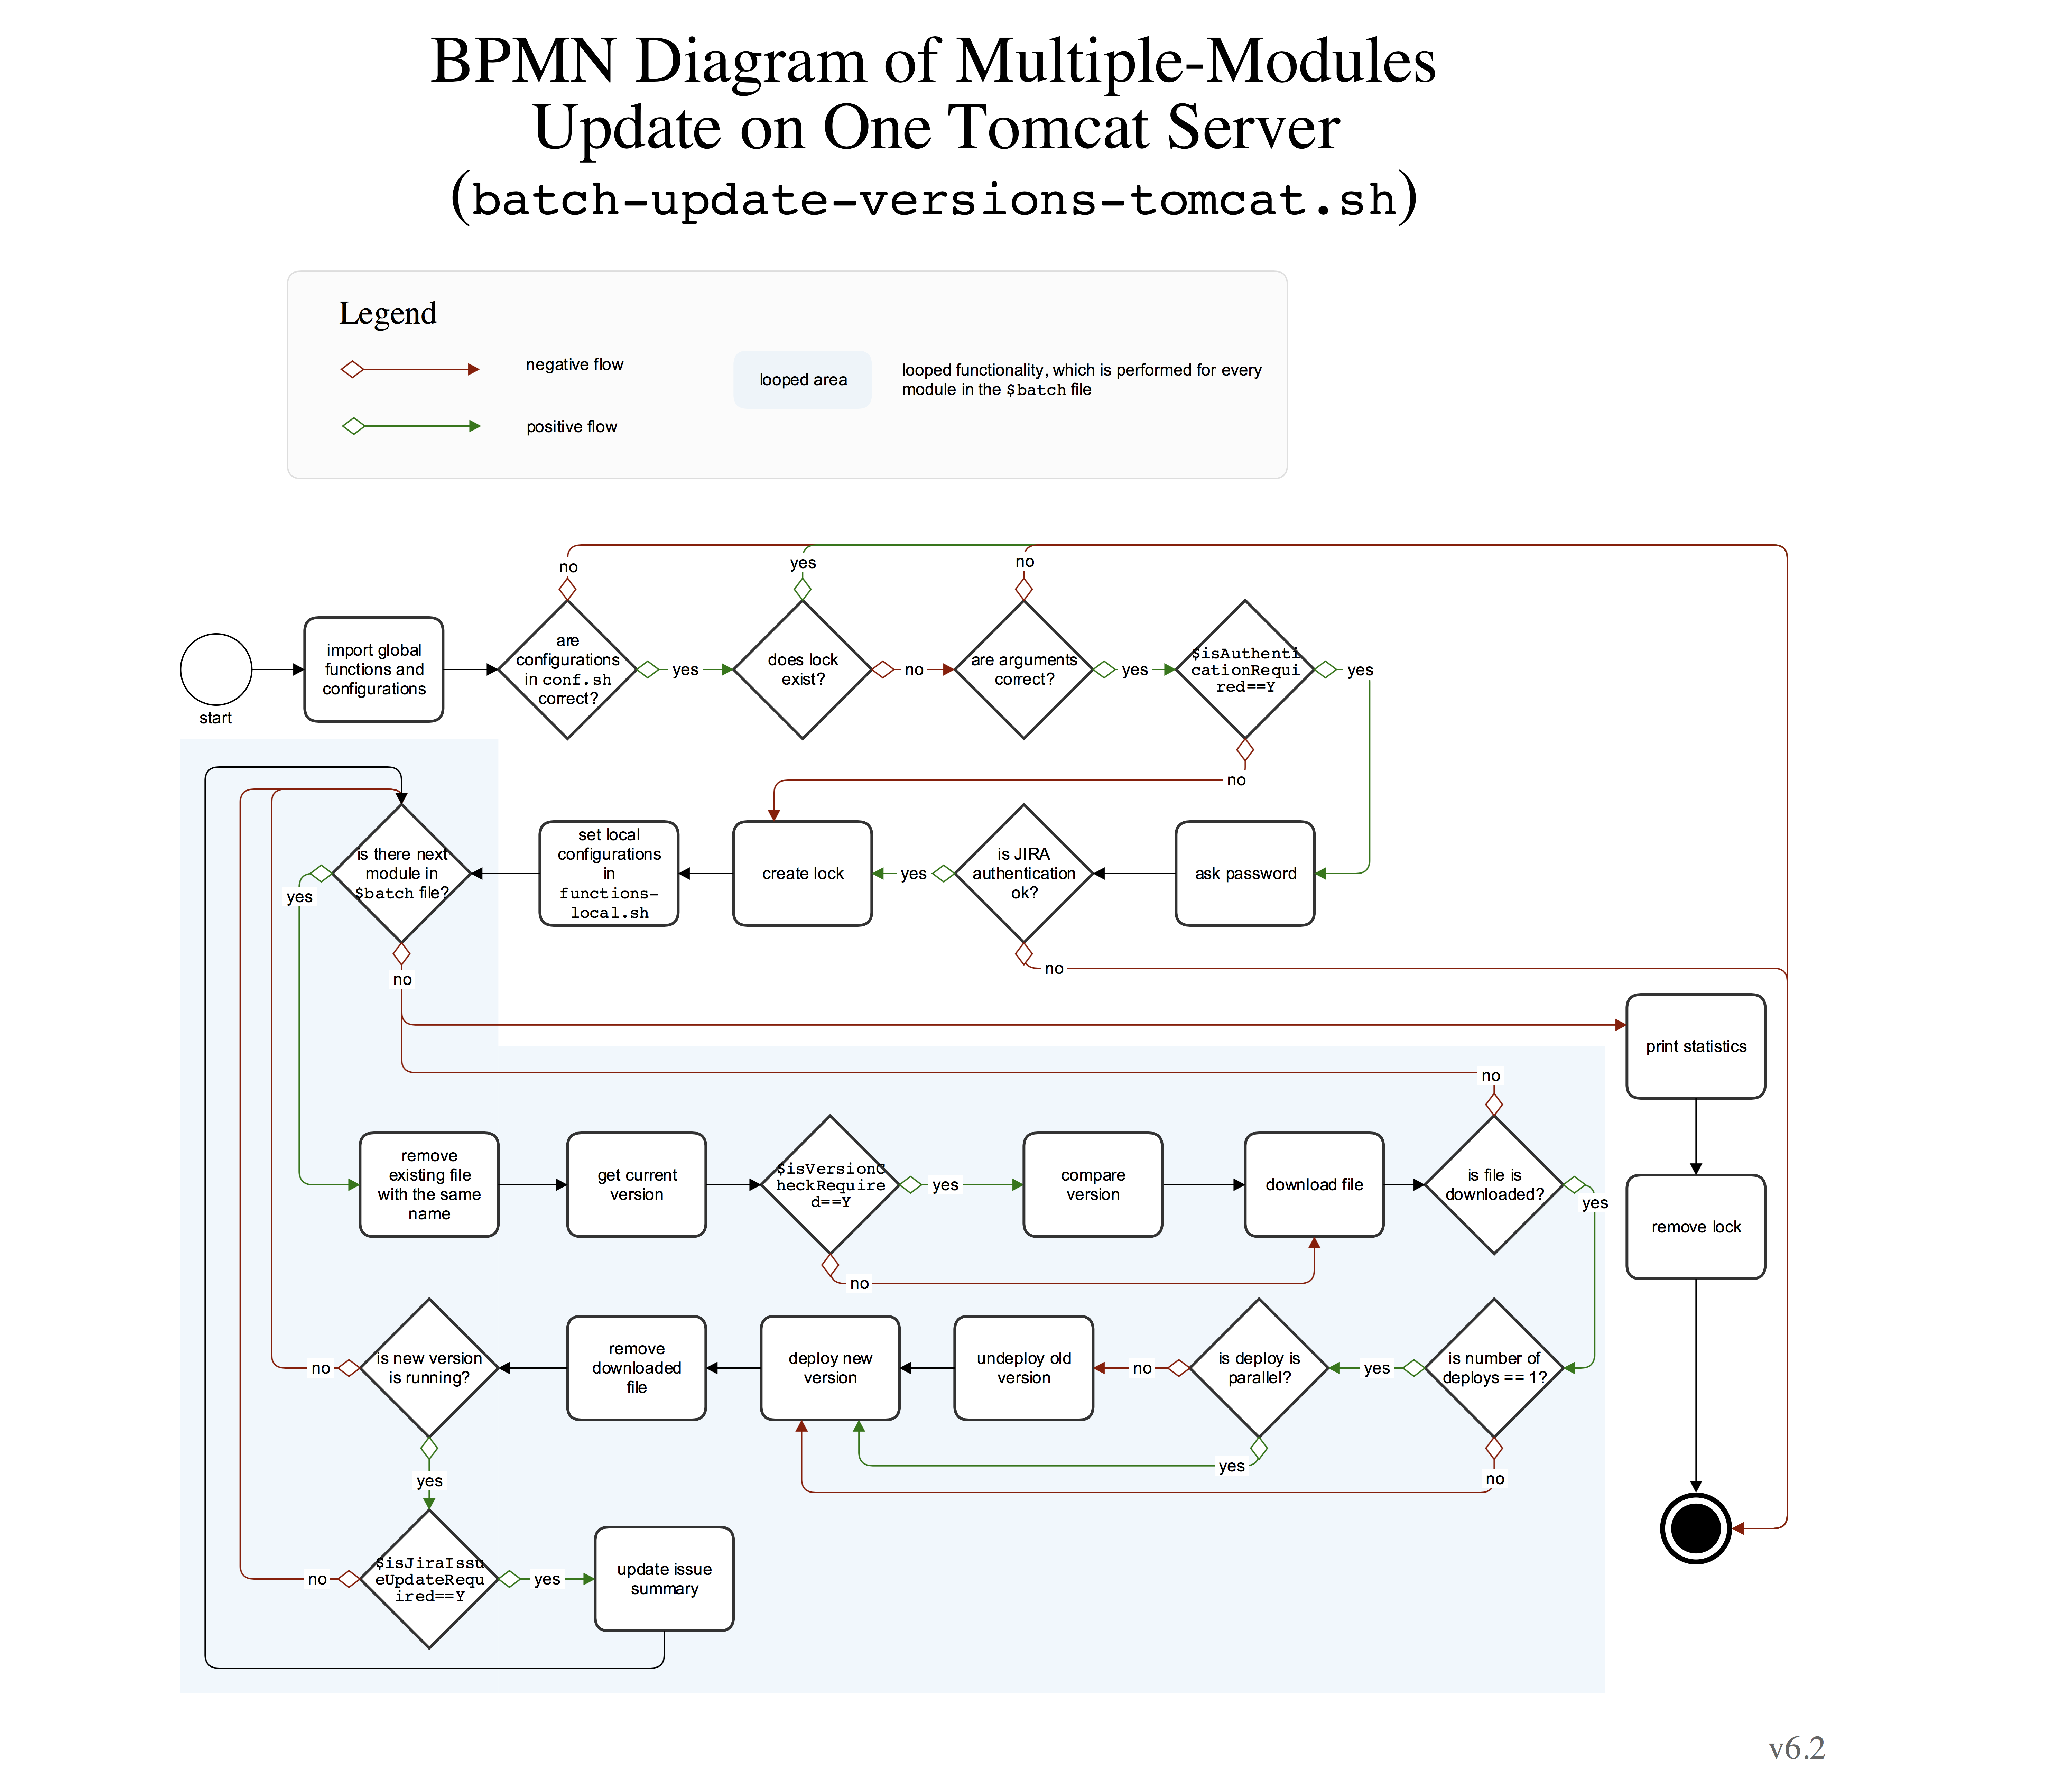
\includegraphics[width=\textwidth]{diagrams/BPMN-diagram-multiple-module-update-tomcat.png}
       \caption*{\textit{Joonis 3. Skripti protsessimudel mitme mooduli uuendamisel Tomcat 8 veebiserveris.}}
     \end{center}
   \end{figure}
   
   \newpage
   
   Olulised funktsioonid, mis on olemas nii mitme kuid ka ühe mooduli uuendamisel, on lukustamine, logimine, teate andmine, kasutaja teavitamine ja ühiste failide sünkroniseerimine.
   
   Lukustamine vastab 8. nõudele Tabelis 2. Töö alguses kontrollib skript, kas serveris eksisteerib lukufail; kui mitte, siis skript tekitab selle ja jätkab tööd. Lukustamise loogika võimaldab vältida paralleelseid uuendusi samas veebiserveris (lukufaili nimetus defineeritakse globaalse muutuja \code{\$lock} abil).
   
   Logimine vastab 6. nõudele \--- skript salvestab logid enda tegevustest (globaalne muutuja \--- \code{\$log}) ning nendest logidest saab teada, kes ja millal mingit moodulit uuendas.
   
   Skript väljastab iga tehtud sammu kohta värvilise teate (Joonis 6). See on seotud nõuetega 1 ja 7: värviline teate aitab kiiremini aru saada uuenduse staatusest (kas see on õnnestunud; kui mitte, siis milline samm ebaõnnestus). See säästab uuendamisprotsessis aega, sest kasutajatel ei ole vaja uurida serveri logifaile, et aru saada, mis sammul protsess katkes. Lisaks kuulub esimese nõude alla ka terminali teavitus (mis teostatakse \code{bell} vahendiga), millega antakse teada, kui skript ootab kasutajalt mingit sisendit (nt JIRA parooli) või kui töö on lõppenud. See tähendab, et kasutaja ei pea uuenduse staatusest aru saamiseks jälgima skripti tööd.
   
   Failide sünkroniseerimine on seotud nõudega 10. Kuna skriptifailid peavad asuma igas serveris, siis on neid vaja parandada ja täiendada mitu korda. Selleks, et vältida töö dubleerimist, asuvad ühised failid (mis vastutavad loogika eest ja ei ole serveri seadistusfailid) repositooriumis. Igas serveris on seadistatud Crontab \cite{cron} tööd, mis kontrollivad regulaarselt, kas repositooriumis on olemas faili uus versioon. Kui see on olemas, siis see laaditakse alla. See tähendab, et skriptiparandusi ja täiendusi on vaja teha ainult üks kord repositooriumis. Joonisel 4 on toodud näide Crontab tööde kirjeldamisest.
   \begin{figure}[H]
     \begin{center} 
       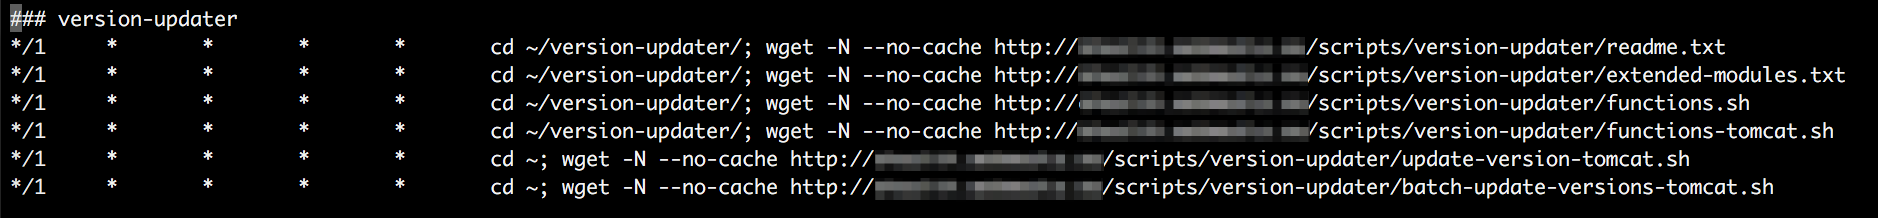
\includegraphics[width=\textwidth]{screenshots/crontab.png}
       \caption*{\textit{Joonis 4. Näide Crontab tööde kirjeldusest ühisfailide automaatseks allalaadimiseks repositooriumist.}}
     \end{center}
   \end{figure}
   
   \newpage
   
    Tabelis 4 on esitatud Bash skripti vastavus kõigile nõuetele Tabelist 2.
   
   \begin{table}[H]
    \caption*{\textit{Tabel 4. Bash uuendamisskripti vastavus nõutele Tabelist 2.}}
    
    \begin{tabular}{|c|p{3.5cm}|p{9.5cm}|}
      \hline
      \textbf{Nr} & \textbf{Nõue} & \textbf{Vastavus}\\
      \hline
      1 & Kiirus. & Uuendamisprotsess võtab varasemast vähem aega \--- selle kohta on toodud statistika peatükis 4.\\
      \hline
      2 & Mugavus. & Uuendamisprotsess nõuab ühe skripti käivitamist. Lisaks on realiseeritud värviline teate ja statistika kuvamine kasutajale.\\
      \hline
      3 & Ühe ja mitme mooduli uuendamine. & On olemas eraldi skriptid ühe ja mitme mooduli uuendamiseks.\\
      \hline
      4 & Töötamine erinevate veebiserveritega. & Lahendus töötab veebiserveritega WebLogic 12 ja Tomcat 8 (vajadusel seda võib kohandada Tomcat 6 ja 7 jaoks).\\
      \hline
      5 & Teavitussüsteem. & Skriptil on kasutusel JIRA tööde uuendamine, mis saadab teavitusi huvitatud inimestele.\\
      \hline
      6 & Logimissüsteem. & On olemas logifail.\\
      \hline
      7 & Mittetehniline lahendus. & Kasutaja ei pea aru saama tehnilistest detailidest, et käivitada skripti sisendparameetritega.\\
      \hline
      8 & Lukustamissüsteem. & Skript tekitab lukufaili töö alguses ja eemaldab seda töö lõpus.\\
      \hline
      9 & Töötamine mitme serveriga. & On olemas funktsioon mitme serveri uuendamiseks.\\
      \hline
      10 & Hallatav lahendus. & Skripti lähtekood on kättesaadav kõigile meeskonnaliikmele ja seda võib  parandada ja täiendada igal hetkel.\\
      \hline
      11 & Kiire arendusprotsess. & Skripti arendamisele ja paigaldamisele kõikidesse rakendustesse kulus umbes 150 tundi.\\
      \hline
      12 & Töötamine moodulite erisufiksitega. & On olemas funktsioon erisufiksitega töötamiseks.\\
      \hline
      13 & Madal hind. & Ühe inimtöö tunnihind projekti jaoks on umbes \euro 45, mis tähendab, et skripti arendus maksis projektile $150 * 45 = $ \euro 6750. Skripti kirjutati osade kaupa: alguses tehti põhisammud 1-5 ja 8 Tabelist 1, hiljem sammud 6-7 ja kõik nõuded Tabelist 2, lõpus koostati täiendavaid funktsioone ja kontrolle, mis lihtsustavad skripti kasutamist ja vähendavad vea tekkimise tõenäosust.\\
      \hline
    \end{tabular}
  \end{table}
  
  \newpage
  
  Skript koosneb 16 failist, mida võib jagada kolme gruppi. Mõned failid on spetsiifilised kas Tomcat või WebLogic veebiserveri jaoks. Mõnede failide nimetusi võib muuta globaalsete muutujate abil. Igas failis on olemas kommentaarid, mis selgitavad faili ja muutujate eesmärke.

  \textbf{Ühised failid} \--- failid, mis on ühised kõigile serveritele (mõned neist sõltuvad veebiserverist) ja mida saab sünkroniseerida:
  
  \begin{itemize}
    \item \code{version-updater/functions.sh} \--- globaalsed üldised funktsioonid, mis ei sõltu veebiserverist;
    \item \code{version-updater/functions-tomcat.sh} \--- globaalsed Tomcat 8 funktsioonid, mida kasutatakse ainult Tomcat veebiserveris;
    \item \code{version-updater/functions-wl.sh} \--- globaalsed WebLogic 12 funktsioonid, mida kasutatakse ainult WebLogic veebiserveris;
    \item \code{deploy-undeploy-script.py} \--- Python skriptid WebLogic veebiserveris moodulite uuendamiseks;
    \item \code{update-version-tomcat.sh} \--- ühe mooduli uuenduse skript, mis sisaldab funktsioonide kasutamise õiget järjekorda Tomcat veebiserveris;
    \item \code{batch-update-versions-tomcat.sh} \--- mitme mooduli uuendamise skript Tomcat veebiserveri jaoks;
    \item \code{update-version-wl.sh} \--- ühe mooduli uuendamise skript WebLogic veebiserveri jaoks;
    \item \code{batch-update-versions-wl.sh} \--- mitme mooduli uuendamise skript WebLogic veebiserveri jaoks;
    \item \code{version-update/extended-modules.txt} \--- nimekiri moodulitest, millel on olemas erinevad sufiksid (nõue 12 Tabelist 2);
    \item \code{version-updater/readme.txt} \--- üldine informatsioon skripti autori ja juhendi kohta.
  \end{itemize}
  
  \textbf{Kohalikud konfiguratsioonifailid} \--- failid, mis sõltuvad serverist, kuhu skript on paigaldatud:
  
  \begin{itemize}
    \item \code{version-updater/conf.sh} \--- konfiguratsioonifail, kus asuvad globaalsed muutujad, mille väärtused sõltuvad serverist, kuhu skript on paigaldatud;
    \item \code{version-updater/functions-local.sh} \--- kohalikud funktsioonid, mis sõltu\-vad serverist;
    \item \code{version-updater/batch-modules.txt} \--- fail, kus kasutaja defineerib moodulite nimetusi ja versioone mitme mooduli uuendamiseks (faili nimetus defineeritakse globaalse muutujaga \code{\$batch});
    \item \code{version-updater/jira-issues.txt} \--- fail, kus on kaardistatud moodulite nimetused ja JIRA tööde koodid (on vajalik ainult JIRA kasutamisel ja on defineeritav globaalse muutujaga \code{\$issues}).
  \end{itemize}
  
  \textbf{Kohalikud väljundfailid} \--- failid, mida skript täidab töö ajal ja mida kasutaja ei tohi muuta:
  
  \begin{itemize}
    \item \code{version-updater/update.log} \--- fail, kus logitakse skripti tegevusi (faili nimetus defineeritakse globaalse muutujaga \code{\$log});
    \item \code{version-updater/jira-rest.txt} \--- tühifail, mida skript kasutab REST \cite{rest} päringute genereerimiseks JIRA töö uuendamisel \cite{jira} (on vajalik ainult JIRA kasutamisel ja on defineeritav globaalse muutujaga \code{\$rest}).
  \end{itemize}
  
  \newpage
  
  Joonisel 5 on toodud näide skriptifailide struktuurist serveris, kus on kasutusel Tomcat 8. Serveri juurkaustas asub alamkaust \code{/tomcat} veebiserveriga, kuhu on paigaldatud moodulid \code{first-module} versiooniga \code{1.2.3.4} ja \code{second-module} versiooniga \code{3.4.5.6}. Skripti uuendamisfailid asuvad rakenduse serveri juurkaustas: \code{batch-update-versions-tomcat.sh} ja \code{update-version-tomcat.sh}. Skripti abifailid asuvad kaustas \code{/version-updater}.
  
  \begin{figure}[H] 
    \begin{center}
      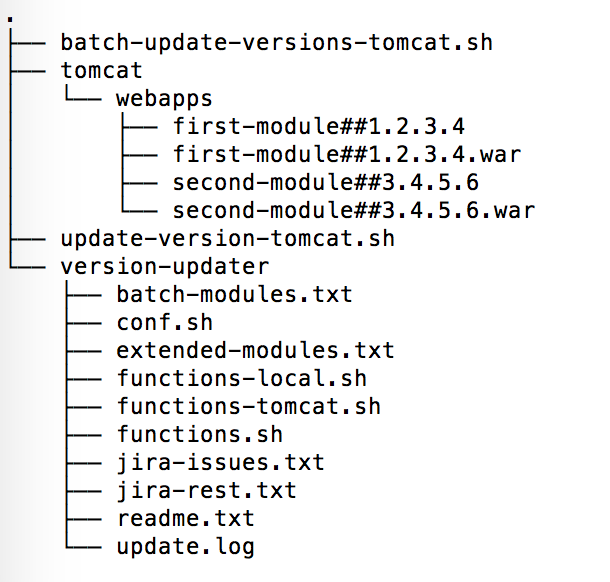
\includegraphics[width=.4\textwidth]{screenshots/file-structure-on-tomcat.png}
      \caption*{\textit{Joonis 5. Skripti failide struktuur veebiserveris Tomcat 8.}}
      \end{center}
   \end{figure}
   
   Lõppkasutajale kasutamiseks mõeldud failid on \code{update-version-*.sh} ja \code{batch-} \code{update-versions-*.sh} (\code{*} asemel on \code{tomcat} või \code{wl}). Lisaks ka logifail \code{update.log} toimunud uuendustest info saamiseks. Kõik ülejäänud failid on mõeldud skripti töö toetamiseks ja seadistamiseks.
   
   \newpage
      
 \subsection{Skripti paigaldamine}
  
  Koodirepositooriumis on olemas kõik skriptifailid, mille saab vajadusel alla laadida serverisse, kohalikku või virtuaalmasinasse. Samuti on olemas zip\--fail, kus on arhiveeritud kõik failid vastavalt skripti versioonile ja veebiserverile (Tomcat ja WebLogic jaoks on eraldi arhiivid). Skripti paigaldamise protsess on kirjeldatud juhendis ja see koosneb neljast sammust:
  \begin{itemize}
    \item vastava zip\--faili allalaadimine serverisse, kohalikku või virutaalmasinasse;
    \item allalaaditud faili lahtipakkimine;
    \item lärgmiste failide väärtustamine serveri\--spetsiifiliste andmetega:
    \begin{itemize}
      \item \code{version-updater/conf.sh};
      \item \code{version-updater/functions-local.sh};
      \item \code{version-updater/jira-issues.txt}.
    \end{itemize}
    \item Crontab tööde seadistamine ühisfailide sünkroniseerimiseks.
  \end{itemize}
  
  Lisaks, Bash skripti kasutamiseks kasutajal peavad olema paigaldatud järgmised vahendid:
  \begin{itemize}
    \item Bash käsureaprotsessor;
    \item veebiserver WebLogic 12 või Tomcat 8;
    \item standardsed UNIX vahendid: \code{find}\footnote{\url{http://www.gnu.org/software/findutils/manual/html_mono/find.html} (12.05.2016)}, \code{grep}\footnote{\url{https://www.gnu.org/software/grep} (12.05.2016)}, \code{wget}\footnote{\url{https://www.gnu.org/software/wget} (12.05.2016)} (kui mooduli failid asuvad veebis), \code{curl}\footnote{\url{https://curl.haxx.se} (12.05.2016)};
    \item standardne käsurea \code{bell} funktsioon.
  \end{itemize}

  \newpage
  
  \subsection{Skripti kasutamine} 
   
  Skripti kasutamiseks piisab ühe faili käivitamist: ühe mooduli uuendamiseks \code{update-version-*.sh} või mitme mooduli uuendamiseks \code{batch-update-}\\
  \code{versions-*.sh} (\code{*} asemel on \code{tomcat} või \code{wl}). Kõiki ülejäänud faile kasutab skript enda töös ja kasutaja ei pea neid käivitama.
  
  Ühe mooduli uuendamise skriptile on võimalik anda neli sisendparameetrit:
  \begin{center}
    \small{\code{./update-version-*.sh MODULE\_NAME MODULE\_VERSION JIRA\_USERNAME [p]}}
  \end{center}
  
  Näide:
  \begin{center}
    \small{\code{./update-version-tomcat.sh admin 1.1.1.1 irina}}
  \end{center}

  \begin{itemize}
    \item \code{MODULE\_NAME} \--- kohustuslik parameeter, mis määrab uuendatava mooduli nimetuse (näiteks Tomcat-i puhul on see sama nimetus, mis tee (\textit{path}) Tomcat Manager-is\footnote{\url{https://tomcat.apache.org/tomcat-7.0-doc/manager-howto.html} (12.05.2016)}).
    \item \code{MODULE\_VERSION} \--- kohustuslik parameeter, mis määrab paigaldatava versiooni numbri.
    \item \code{JIRA\_USERNAME} \--- parameetrit tuleb kasutada siis, kui JIRA autentimine on kohustuslik (globaalne muutuja \code{\$isAuthenticationRequired="Y"}).
    \item \code{p} \--- mittekohustuslik parameeter, mille sisestamisel teostatakse paralleelne uuendus\footnote{\url{https://tomcat.apache.org/tomcat-8.0-doc/config/context.html\#Parallel\_deployment} (12.05.2016)} (ei toimu vana versiooni eemaldamist).
  \end{itemize}\\
  
  Mitme mooduli uuendamise skriptile on võimalik anda kaks sisendparameetrit:
  
  \begin{center}
    \small{\code{./batch-update-versions-*.sh JIRA\_USERNAME [p]}}
  \end{center}
  
  Näide:
  \begin{center}
    \small{\code{./batch-update-versions-tomcat.sh irina p}}
  \end{center}
  
    Sisendparameetrid \code{JIRA\_USERNAME} ja \code{p} on samad, mis ühe mooduli uuendamise korral.
  
  Joonisel 6 on näidatud ühe mooduli edukas uuendus. Skript annab teate kõigist sooritatud sammudest.
  
  \begin{figure}[H]
     \begin{center} 
       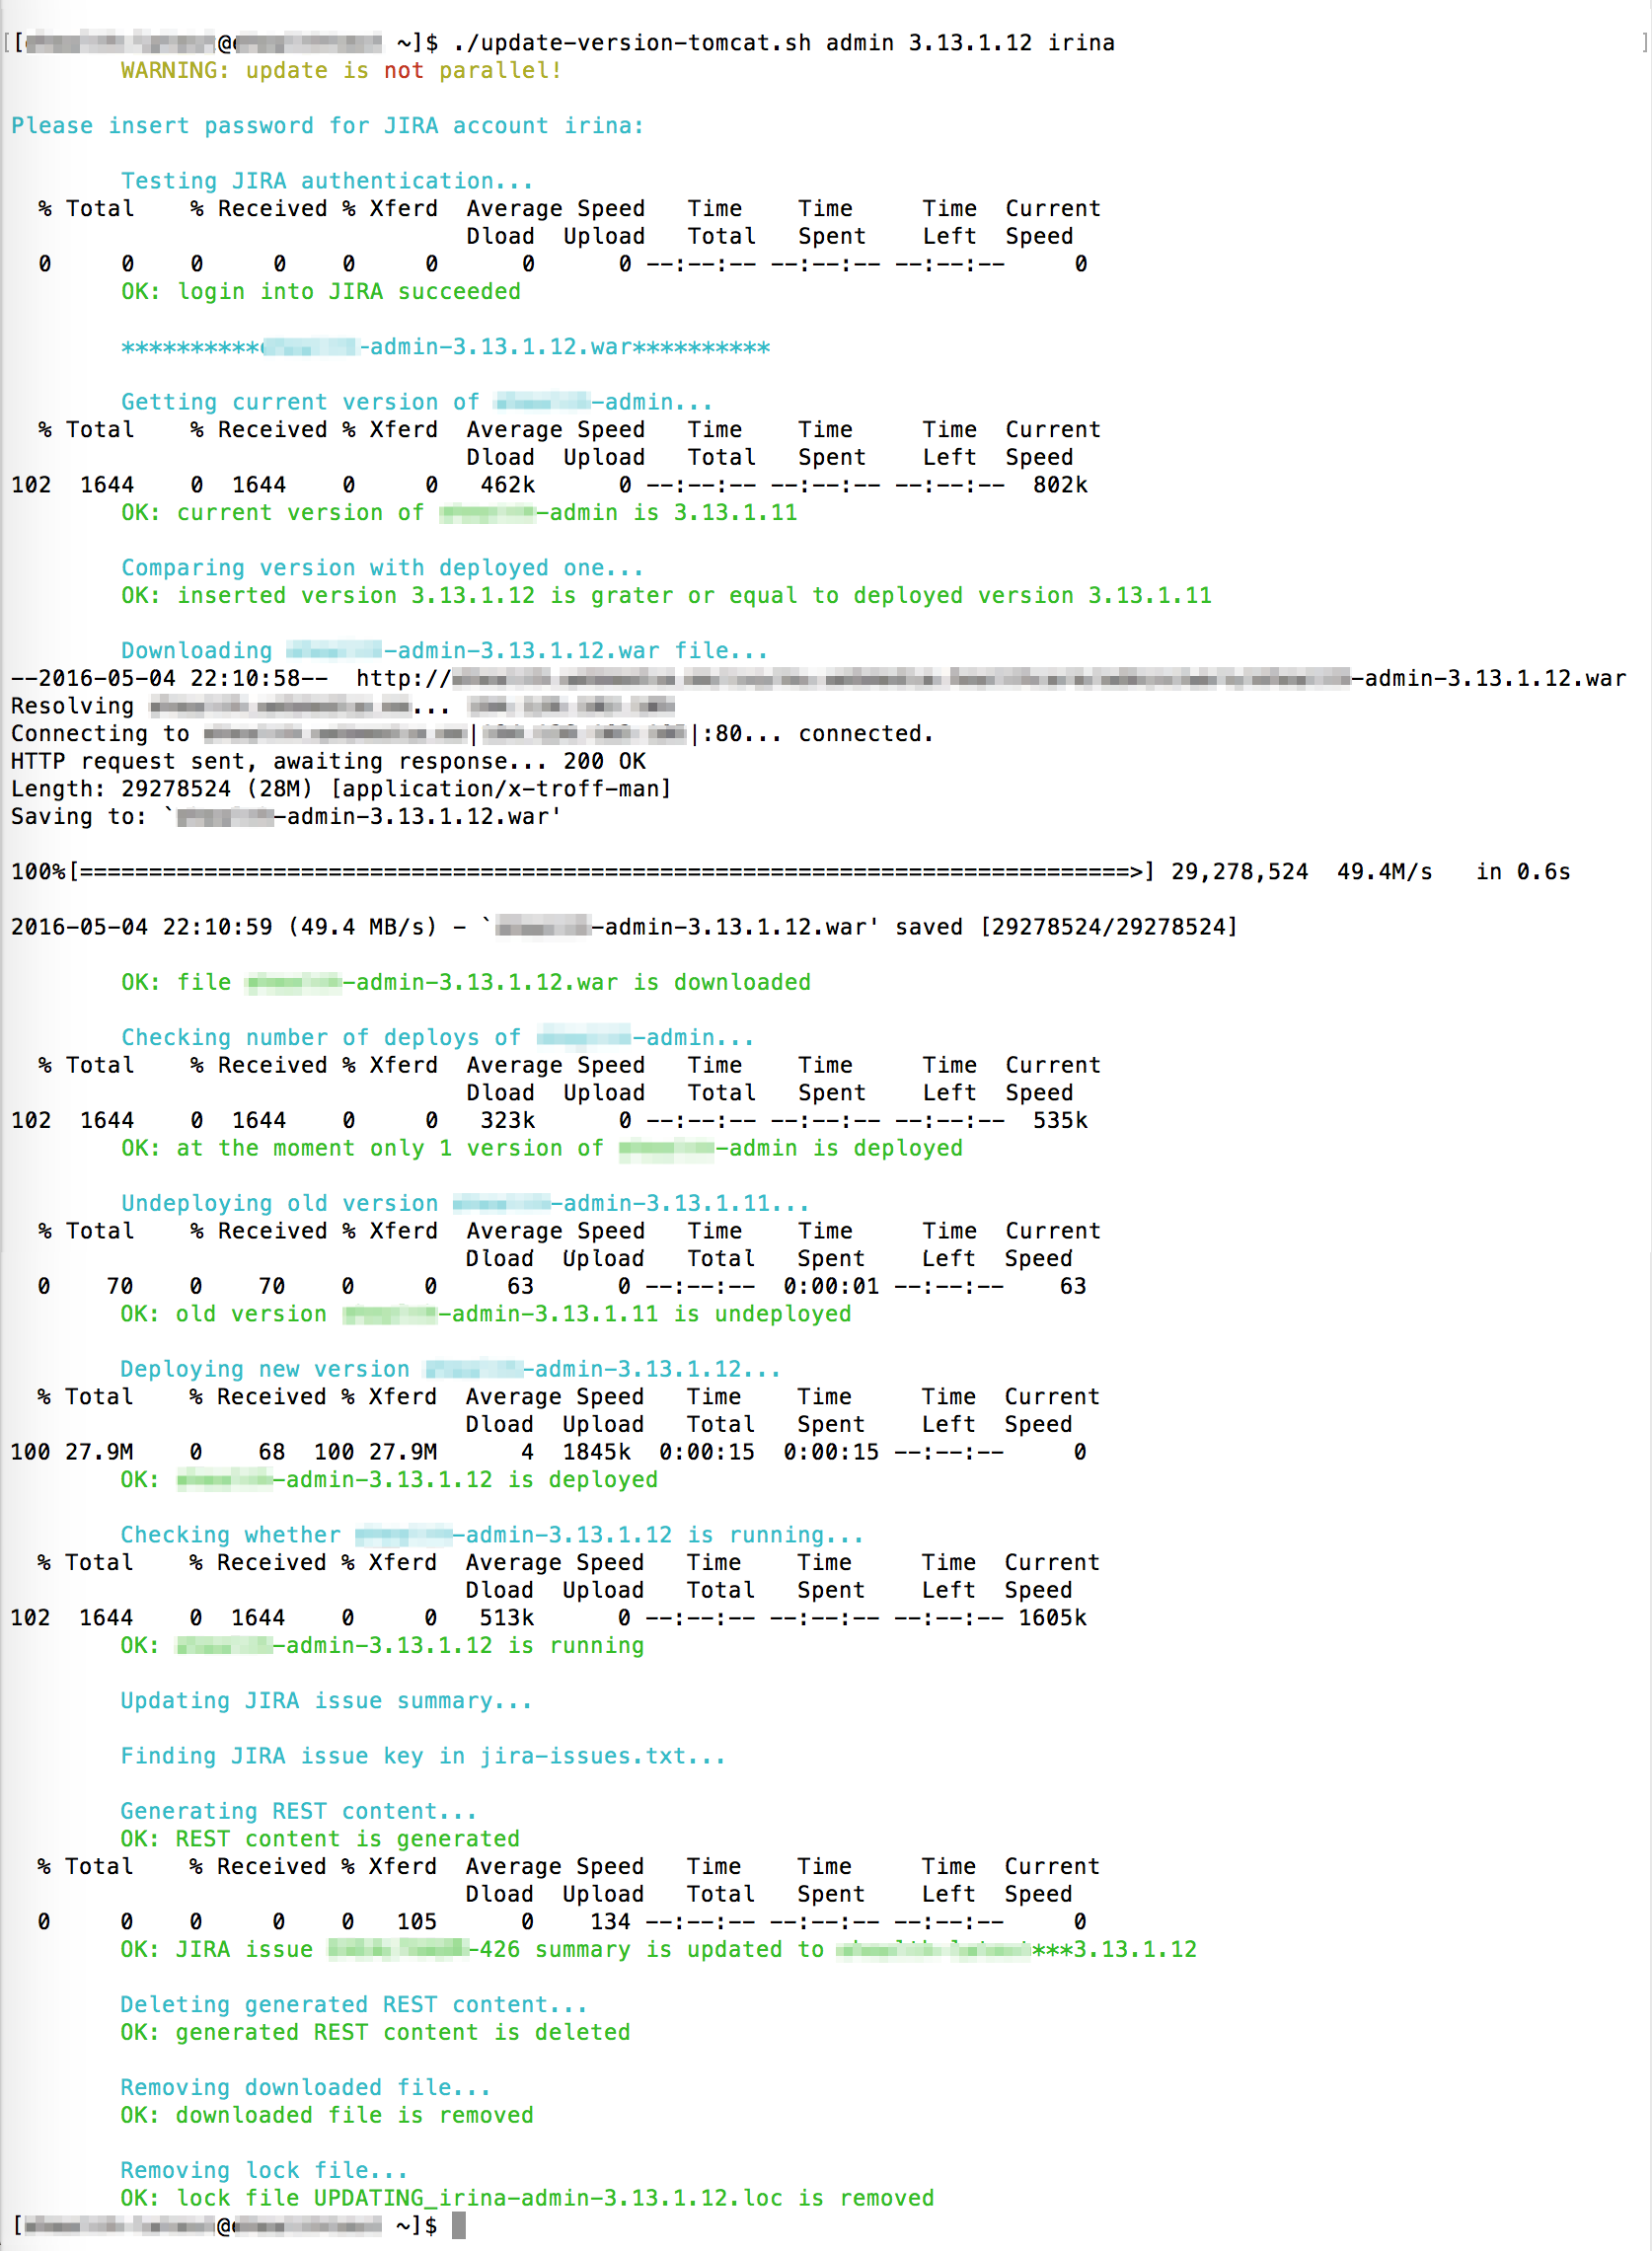
\includegraphics[width=.85\textwidth]{screenshots/one-module-successful-update.png}
       \caption*{\textit{Joonis 6. Ühe mooduli edukas uuendamine skripti abil.}}
     \end{center}
  \end{figure}
  
  \subsection{Dokumentatsioon}
  
  Skripti kohta on olemas dokumentatsioon, mis on uuendamise oluline osa. Skripti juhend kirjeldab, kuidas skripti on võimalik kasutada, paigaldada ja seadistada. Juhend on kättesaadav kõigile meeskonnaliikmetele, mis tähendab, et igaühel on võimalus seda kasutada. Nii skripti projektisisene juhend kui ka avalik juhend on ära toodud töö Lisades IV ja V.
  
  \newpage
  
  % Mõju projektile
  \section{Uue lahenduse mõju projektile}
  
  Automaatne versiooniuuendus asendas täielikult vana käsitsiprotsessi. Sellel on olemas nii oma eelised kui ka puudused.
  
  Kõige olulisem eelis on see, et skript täidab kõik Tabelis 2 esitatud nõuded, neist enim väärivad märkimist nõuded 1 ja 2 \--- protsessi kiirus ja mugavus.
  
  Töö käigus mõõdeti vana ja uue uuendamisprotsessi kiirust. Automaatse protsessi alguseks loeti skripti käivitamise käsku ja lõpuks skripti teavitust töö lõpetami\-sest. Skripti tööaja mõõtmiseks kasutati UNIX käsurea funktsiooni \code{time}\footnote{\url{http://pubs.opengroup.org/onlinepubs/9699919799/utilities/time.html} (12.05.2016)}. Käsitsi uuendamisprotsess koosneb sammudest, mida kirjeldati Tabelis 1 ja sellele kulunud aega mõõdeti stopperiga.
  
  Valiti neli protsessi, mis teostati samas serveris ja samade war\--failidega: kolme kõige populaarsema mooduli eraldi uuendamine ja kõigi moodulite uuendamine (valitud rakenduses oli neid 18). Iga protsess sooritati käsitsi ja automaatselt kolmel korral, võrdlemiseks kasutati katsete keskmisi väärtusi. Tulemused on toodud Tabelis 5.
  
  \begin{table}[!htbp]
    \begin{center}
      \caption*{\textit{Tabel 5. Vana ja uue meetodi tööaeg.}}
      
      \begin{tabular}{| l | c | c | c | c |}
        \hline
         \textbf{Moodul} & \textbf{Automatiseeritud} & \textbf{Käsitsi} & \textbf{Uuendusi} & \textbf{Säästetud aeg}\\
         \textbf{} & \textbf{uuendus} & \textbf{uuendus} & \textbf{2015. aastal} & \textbf{2015. aastal}\\
        \hline
        admin & 27s & 80s & 67 tk & 1t\\
        treatment & 61s & 112s & 240 tk & 3t 44m\\
        reception & 38s & 100s & 197 tk & 3t 39m \\
        kõik (18 tk) & 552s & 1048s & \--- & \---\\
        \hline
      \end{tabular}
    \end{center}
  \end{table}
  
  Kaks viimast veergu näitavad säästetud aega 2015. aastal (terve aasta kasutati uuendamiseks automaatset skripti). Veerus ``Uuendusi 2015. aastal'' on toodud vastava mooduli uuenduste arv valitud testrakenduses aasta jooksul. Veerus ``Säästetud aeg 2015. aastal'' on ära näidatud 2015. aastal kokkuhoitud aeg, mis on saadud käsitsi ja automaatse uuendamise aja erinevuse korrutamisel uuenduste arvuga.
  
  Tegelikkuses on kokkuhoitud aeg veelgi suurem, sest vana protsess nõudis tähelepanu kogu protsessi vältel. Uut skripti kasutades saavad kasutajad tegeleda paralleelselt teiste ülesannetega ega ei pea jälgima skripti tööd (skript annab ise teada kui uuendamine on lõpule viidud).
  
  Peamiseks puuduseks on, et kasutajad ei tunne enam versiooniuuenduse protsessi tausta ja vigade tekkimisel (kas tingituna serverist, veebiserverist või skriptist) ei oska neid parandada. See on üldine automatiseerimise probleem, millega tuleb mugavuse nimel leppida.
  
   Käesoleva töö raames küsiti tagasisidet automatiseeritud uuendamisprotsessi kohta seda kasutanud meeskonnaliikmetelt. Allpool on toodud mõned väljavõtted, terviktekstid on kättesaadavad Lisas VI.
   
   \begin{displayquote}
   ``I also like that scalability has been considered when writing the script + many optional features have been implemented which can be used if one desires to do so.'' (Martin Rakver, Hosting Services and Application Manager)
   \end{displayquote}
   
   \begin{displayquote}
   ``I personally think that version-update script has significantly improved the speed of version update.'' (Kalle Jagula, QA Specialist)
   \end{displayquote}
   
   \begin{displayquote}
    ``Version updater script has standardized the way our environments are updated, reducing learning curve for new people performing the task. Downside is that people are unaware, what happens in the background and can't handle simple errors in the process anymore.'' (Tanel Käär, System Architect)
    \end{displayquote}
    
    \begin{displayquote}
    ``The scripts allowed me to conveniently perform the updates while letting me concentrate on solving the primary problems and not leaving the environment containing all necessary information.'' (Klaus-Eduard Runnel, Senior Programmer)
    \end{displayquote}
    
    \begin{displayquote}
    ``Samuti tooks välja, et uuendamise skriptid on väga hästi dokumenteeritud ja põhjalikult kirja pandud kuidas toimivad.'' (Helina Ziugand, QA Specialist)
    \end{displayquote}

  \newpage
  
  % Lahenduse edasiarendamine
  \section{Lahenduse edasiarendamine}
  
  Lähitulevikus planeeritakse lahendada skripti põhiprobleemi, mis seisneb selles, et kasutajad ei tunne versiooniuuendamise protsessi ja ei oska parandada uuendamise ajal tekkivaid vigu. Selleks lisatakse skriptile  funktsioon, mis loeb serveri ja veebiserveri logid, leiab sealt tekkinud vea põhjuse, selgitab seda inimkeeles ja pakub kasutajale vastava lahenduse.
  
  Samuti planeeritakse realiseerida kolleegi soovitus samaaegsest mitme rakenduse uuendamisest, selleks et ühekorraga uuendada samad moodulid ja samad versioonid mitmel rakendusel.
  
  Kaugtulevikus planeeritakse tsentraliseerida skripti, et iga rakenduse uuendamine toimuks ühest kohast ja uuendamiseks ei oleks vaja siseneda igasse serverisse eraldi.
  
  Lisaks projektisisestele plaanidele oodatakse skripti parandusi ja täiendusi GitHub kogukonnast, kuna Bash skripti kood on avalik (ainult Apache Tomcat veebiserverile) ja asub GitHub repositooriumis (Lisa VII). See tähendab, et igaüks, kellel on sarnane tarkvaraarenduse süsteem, saab seda kasutada ja täiendada vastavalt oma nõuetele. Igas failis on kommentaarid, mis selgitavad faili eesmärke ja kasutamisviisi. Samuti on GitHub platvormil olemas võimalus vigadest teatamiseks ja uute funktsioonide tellimiseks.
  
  Skripti rakendamise lihtsustamiseks on olemas avalik dokumentatsioon, mis asub GitBook repositooriumis. See sisaldab kasutusjuhendit, paigaldamise ja seadistamise juhendit ning kirjeldab, kuidas on võimalik skripti tööd UNIX standardsete vahenditega laiendada.
  
  \newpage
  
  % Kokkuvõte
  \section*{Kokkuvõte}
  \label{kokkuvote}
  \addcontentsline{toc}{section}{\nameref{kokkuvote}}
  
  Käesoleva bakalaureusetöö eesmärgiks oli automatiseerida versiooniuuenduse protsessi konkreetses projektis, et säästa aega ja vähendada inimlike vigade arvu.
  
  Bakalaureusetöö teoreetilise osa käigus sõnastati probleemi lahendusele 13 nõuet ja uuriti nelja erinevat tööriista versiooniuuenduste haldamiseks. Mitte ükski neist ei vastanud kõigile nõuetele. Lahenduseks valiti Bash skripti kirjutamine.
  
  Bakalaureusetöö praktilise osa käigus kirjutati versioonide uuendamiseks Bash skript, mis vastab kõigile nõuetele. Samuti koostati juhend selle skripti paigaldamiseks, seadistamiseks ja kasutamiseks.
  
  Kokkuvõtteks võib öelda, et bakalaureusetöös püstitatud eesmärgid on täidetud. Kirjutatud Bash skript aitab kiiremini ja mugavamalt projektis versioone uuendada. Seda kinnitavad nii meeskonnaliikmete tagasiside kui ka käsitsi ja automatiseeritud protsessi kiiruse võrdlemine.
  
  Loodud lahendust saavad kasutada ja täiendada ka teised arendajad, sest lahenduse kood ja dokumentatsioon on avalikult kättesaadavad.

  \newpage
  
  % Kasutatud materjalid 
  \begin{thebibliography}{9}
    \label{kasutatud-materjalid}
    \addcontentsline{toc}{section}{\nameref{kasutatud-materjalid}}
    
    \bibitem{bamboo}
    Atlassian Bamboo koduleht. [Veebis, 5.05.2016].\\
    \url{https://www.atlassian.com/software/bamboo}
    
    \bibitem{chef}
    Chef Delivery koduleht. [Veebis, 5.05.2016].\\
    \url{https://www.chef.io}
  
    \bibitem{jenkins}
    Jenkins koduleht. [Veebis, 5.05.2016].\\
    \url{https://jenkins.io}
  
    \bibitem{ansible}
    Ansible Tower koduleht. [Veebis, 5.05.2016].\\
    \url{https://www.ansible.com}
  
    \bibitem{bash}
    Bash-keele kasutusjuhend. [Veebis, 5.05.2016].\\
    \url{https://www.gnu.org/software/bash/manual/bashref.html}
    
    \bibitem{bash-book}
     Stephen G. Kochan ja Patrick Wood, ``Unix Shell Programming,'' \textit{Sams Publishing}, 2003
     
     \bibitem{cron}
    Crontab-vahendi kasutusjuhend. [Veebis, 5.05.2016].\\
    \url{https://help.ubuntu.com/community/CronHowto}
    
    \bibitem{rest}
    Todd Fredrich, ``RESTful Service Best Practices,'' \textit{Pearson eCollege}, mai 2012.\\
    \url{http://www.restapitutorial.com/media/RESTful_Best_Practices-v1_1.pdf}
    
    \bibitem{jira}
    JIRA REST API Reference. [Veebis, 5.05.2016].\\
    \url{https://docs.atlassian.com/jira/REST/latest}
 
  \end{thebibliography}

  \newpage
  
  % Lisad
  \section*{Lisad}
  \label{lisad}
  \addcontentsline{toc}{section}{\nameref{lisad}}
  
  \subsection*{I Terminid}
  \label{terms}
  \addcontentsline{toc}{subsection}{\nameref{terms}}
  
  \textbf{Demorakendus} \--- rakendus, mida kliendid kasutavad funktsioonide testimiseks.\\
  
  \textbf{Moodul} \--- tarkvara osa, kuhu on kogutud ja pakitud ühe funktsiooni kood (üks war\--fail on üks moodul).\\
  
  \textbf{Modulaarne süsteem} \--- tarkvaraarenduse süsteem, mille korral kogu kood jagatakse moodulitesse, et ühe funktsiooni tarnimine ei nõuaks terve rakenduse uuendamist.\\
  
  \textbf{Rakendus (\textit{application})} \--- tarkvara, mis on paigaldatud veebiserverisse ja on kättesaadav kasutamiseks.\\
  
  \textbf{Server} \--- riist- ja tarkvarasüsteem, kuhu on paigaldatud veebiserver.\\
  
  \textbf{Testrakendus} \--- rakendus, mida projekti meeskonnaliikmed kasutavad tarkvara testimiseks.\\
   
  \textbf{Toodangrakendus} \--- lõppkasutajatele mõeldud rakendus.\\
  
  \textbf{Veebiserver} \--- klient-server-mudelil ja protokollil HTTP või HTTPS põhinev tarkvara, mis võtab vastu kasutajate brauseritelt tulevaid päringuid ja saadab vastuseks HTML-lehti ja faile (nt Apache Tomcat või Oracle WebLogic)\footnote{\url{http://akit.cyber.ee/term/3152-veebiserver} (12.05.2016)}.\\
  
  \textbf{Versioon} \--- number, mis määrab war\--faili sisu (war\--fail sisaldab funktsionaalsust ja parandusi vastavalt versiooni numbrile).\\
  
  \textbf{Versiooniuuendamine} \--- protsess, mille korral veebiserverisse paigaldatakse mooduli uuemat versiooninumbrit, selleks, et rakendada selle parandusi või täiendusi.\\
  
  \newpage
  
  \subsection*{II Ühe mooduli uuendamise mudel}
  \label{bpmn-one}
  \addcontentsline{toc}{subsection}{\nameref{bpmn-one}}
  
  Skripti protsesside mudel ühe mooduli uuendamisel Tomcat 8 veebiserveril asub avalikus GitHub repositooriumis:\\
  \url{https://raw.githubusercontent.com/iriiiina/bachelors-thesis/master/thesis/diagrams/BPMN-diagram-one-module-tomcat.png}
  
  \subsection*{III Mitme mooduli uuendamise mudel}
  \label{bpmn-many}
  \addcontentsline{toc}{subsection}{\nameref{bpmn-many}}
  
  Skripti protsesside mudel mitme mooduli uuendamisel Tomcat 8 veebiserveril asub avalikus GitHub repositooriumis:\\
  \url{https://iriiiina.gitbooks.io/version-updater-manual/content/BPMN-diagram-multiple-module-update-tomcat.png}
  
  \subsection*{IV Skripti projektisisene juhend}
  \label{documentation}
  \addcontentsline{toc}{subsection}{\nameref{documentation}}
  
  Bash skripti projektisisene juhend:\\
  \url{https://github.com/iriiiina/bachelors-thesis/blob/master/manual/Confluence%20Manual.pdf}
  
  \subsection*{V Skripti avalik juhend}
  \label{public-documentation}
  \addcontentsline{toc}{subsection}{\nameref{public-documentation}}
  
  Bash skripti avalik juhend asub avalikus GitBook repositoorimus:\\
  \url{https://iriiiina.gitbooks.io/version-updater-manual/content/}
  
  \subsection*{VI Kolleegide tagasiside}
  \label{feedback}
  \addcontentsline{toc}{subsection}{\nameref{feedback}}
  
  \textbf{Martin Rakver, Hosting Services and Application Manager}
  
  \begin{displayquote}
  I have not been using the script very much, because I rarely update modules nowadays. But what I can say is that it is definately in the right place – automating activities that testers would need do to on daily basis each time when deploying a new module. Come to think about it, there are actually quite many activites related to new module deployment – would be interesting to compare the time it takes to deploy a module manually vs using script + calculate about how much time we as a team are saving daily, montly, yearly (and get to do more important things with that time).
I also like that scalability has been considered when writing the script + many optional features have been implemented which can be used if one desires to do so.
  \end{displayquote}
  
  \newpage

  \textbf{Kalle Jagula, QA Specialist}
  
  \begin{displayquote}
  I personally think that version-update script has significantly improved the speed of version update. Especially with the settings for bulk-update, which improves the speed of modules' version update and manageability of test/demo environments.
  \end{displayquote}
  
  \textbf{Tanel Käär, System Architect}
  
  \begin{displayquote}
  Version updater script has standardized the way our environments are updated, reducing learning curve for new people performing the task. Downside is that people are unaware, what happens in the background and can't handle simple errors in the process anymore.
  \end{displayquote}
  
  \textbf{Klaus-Eduard Runnel, Senior Programmer}
  
  \begin{displayquote}
  I have mostly used the scripts to perform quick module and dependency updates in specific test environments when deploying quick fixes or debugging problems in the modules I'm responsible for. Deployment of artifacts is secondary task in such scenarios. The scripts allowed me to conveniently perform the updates while letting me concentrate on solving the primary problems and not leaving the environment containing all necessary information.

In some cases it was necessary to deploy custom-built experimental (unversioned) war-files. In these cases the scripts could not be used.
They would have been useful though if such experiments would have been commited to feature branches and published as feature branch artifacts. (As of today, we are better prepared for such circumstances.)

The scripts were also useful to deploy predefined sets of modules to temporary test environments living on reusable virtual machine images. It is important to note that a module update triggers launching a set of associated sql scripts to bring a database schema up to date. In that way the version update scripts let us automate most of a process of setting up updated environment from virtual machine images.

It would be helpful if the scripts were adapted to perform changes on remote machines and to perform changes on multiple environments simultaneously.
  \end{displayquote}
  
  \newpage

  \textbf{Helina Ziugand, QA Specialist}
  
  \begin{displayquote}
  Uuendamise skriptid on nii projektile kui ka minu igapäevasele tööle väga positiivselt mõjunud. 
Kui algselt oli uuendamise jaoks vaja mitu sammu käsitsi teha, siis nüüd käib see automaatselt ja kiiresti. Võiks öelda, et üsna tüütu oli alguses kogu see uuendamise protsess - pidevalt pidi jälgima, kas vaja käsureale kirjutada järgmist sammu, hiljem JIRAs vana versiooni numbrit muuta ja Weblogicust vana versioon kustutada. Praegu on väga mugav ühe käsklusega uuendamise skript tööle panna, mis korraga kõik vajalikud sammud ära teeb ja samal ajal kui skript jookseb ise teiste tegevustega jätkata. Väga selgelt erinevate värvidega on välja tootud error, warningu ja success teated, mis on lihtsasti märgatavad ja hästi loetavad.

Kui vaja on rohkem kui ühte moodulit uuendada, siis väga hea lahendus on selleks mitme moodulise uuendamise skript. Kui varem oli vaja rakenduse uue tsükli peale uuendada, siis võttis see ebamugavalt kaua aega ja vabatahtlikult kõige parema meelega seda ette ei tahtnud võtta. Nüüd on vaja ainult uuendatavad versioonid tekstifaili kirja panna ja ühe käsklusega skript käima tõmmata. 

Samuti tooks välja, et uuendamise skriptid on väga hästi dokumenteeritud ja põhjalikult kirja pandud kuidas toimivad. Mul on väga hea meel, et versioonide uuendamine on skriptide abil nii lihtsaks, mugavaks ja meeldivaks tegevuseks saanud.'
  \end{displayquote}
  
  \subsection*{VII Skripti lähtekood}
  \label{source-code}
  \addcontentsline{toc}{subsection}{\nameref{source-code}}
  
  Bash skripti kood asub avalikus GitHub repositooriumis:\\
  \url{https://github.com/iriiiina/version-updater}
  
  \newpage

  \subsection*{VIII Litsents}
  \label{licence}
  \addcontentsline{toc}{subsection}{\nameref{licence}}
  
  \textbf{Lihtlitsents lõputöö reprodutseerimiseks ja lõputöö üldsusele kättesaadavaks tegemiseks}\\
  
  Mina, \textbf{Irina Ivanova}, (sünnikuupäev: 9.05.1988)
  \begin{enumerate}
    \item annan Tartu Ülikoolile tasuta loa (lihtlitsentsi) enda loodud teose \textbf{Versiooniuuenduse automatiseerimine kasutades skriptimiskeelt Bash}, mille juhendajad on Helle Hein ja Polina Morozova,
    \begin{enumerate}
      \item reprodutseerimiseks säilitamise ja üldsusele kättesaadavaks tegemise eesmärgil, sealhulgas digitaalarhiivi DSpace-is lisamise eesmärgil kuni autoriõiguse kehtivuse tähtaja lõppemiseni;
      \item üldsusele kättesaadavaks tegemiseks Tartu Ülikooli veebikeskkonna kaudu, sealhulgas digitaalarhiivi DSpace-i kaudu kuni autoriõiguse kehtivuse tähtaja lõppemiseni.
    \end{enumerate}
    \item olen teadlik, et punktis 1 nimetatud õigused jäävad alles ka autorile.
    \item kinnitan, et lihtlitsentsi andmisega ei rikuta teiste isikute intellektuaalomandi ega isikuandmete kaitse seadusest tulenevaid õigusi.
  \end{enumerate}
  
  Tartus, 1.05.2016

\end{document}